% Clinical ratings

\lecture{Application: Clinical Ratings}{Clinical}

\begin{frame}
	\frametitle{Clinicians disagree in AandE}
	\begin{itemize}
		\item Patients in \ac{AE} are continually monitored.
		\begin{itemize}
			\item Heart rate
			\item Blood pressure
			\item Temperature
			\item etc
		\end{itemize}
		\item<2-> Based on these hourly observations, clinicians (in a Glasgow hospital) give each patient an ordinal rating
		\begin{itemize}
			\item A (healthy(ish)), B, C, D, E, F (critical)
		\end{itemize}
		\item<3->These ratings are \emph{subjective}
		\begin{itemize}
			\item How do clinicians disagree? (variance? bias?)
		\end{itemize}
		\item<3->More details of this work in \href{http://dx.doi.org/10.1109/JBHI.2013.2252182}{Rogers et al 2013} and \href{http://dx.doi.org/10.1007/s11222-009-9125-z}{Rogers et al 2010}
	\end{itemize}
\end{frame}

\begin{frame}
	\frametitle{Data}
	\begin{itemize}
		\item $c = 1\ldots C$ clinicians.
		\item $p=1\ldots P$ patients.
		\item For patient $p$, we have $T_p$ observations at times $\mathbf{t}_p = [t_{p1},\ldots,t_{pT_p}]^T$.
		\item $y_{\tau c}^p$ is rating at $t_{p\tau}$ ($\{A,B,C,D,E\}$).
	\end{itemize}
\end{frame}

\begin{frame}
	\frametitle{The model}
		\begin{itemize}
		\item Assumptions:
			\begin{itemize}
				\item We assume that there is an unobserved continuous latent health function for each patient
				\item Each clinician observes this and and corrupts it in two ways:
					\begin{itemize}
						\item Adds Gaussian noise
						\item Adds a constant offset (optimist, pessimist)
					\end{itemize}
				\item Corrupted health is then binned to give category
			\end{itemize}
		\item<2-> The model:
		\begin{itemize}
			\item Patient health is modelled as a GP.
			\item Corrupted health is the auxiliary variable ($q$)
			\item $q$ is binned to produce rating.
			\item Note that $p(q|f)$ has been generalised from standard normal.
		\end{itemize}
	\end{itemize}
\end{frame}

\begin{frame}
	\frametitle{Model}
	\begin{multicols}{2}
		\begin{figure}[tbh]
			\centering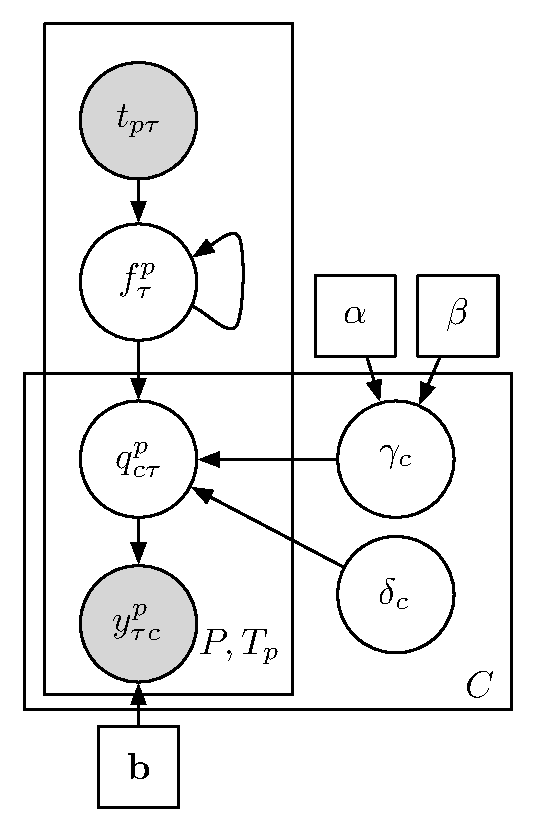
\includegraphics[width=0.9\linewidth]{ClinicalCartoon.pdf}
			\centering\caption{\label{fig:clincartoon}Plates diagram}
		\end{figure}
		\newpage
		\begin{eqnarray}
			\nonumber \blf^p &\sim & {\cal N}(\mathbf{0},\mathbf{C}^p)~~\mbox{[health]}\\
			\nonumber \delta_c &\sim & {\cal N}(0,1)~~\mbox{[offset]}\\
			\nonumber \gamma_c &\sim & {\cal G}(\alpha,\beta)~~\mbox{[precision]}\\
			\nonumber q_{c\tau}^p &\sim & {\cal N}(f_\tau^p + \delta_c,\gamma_c^{-1})\\
			\nonumber P(y_{\tau c}^p=k) &=& \delta(b_k < q_{c\tau}^p < b_{k+1})
		\end{eqnarray}
		Previously auxiliary variables were $z_n\sim {\cal N}(f_n,1)$. This model adds clinician-specific offsets and precisions: $q_{c\tau}^p \sim  {\cal N}(f_\tau^p + \delta_c,\gamma_c^{-1})$.
	\end{multicols}
\end{frame}

\begin{frame}
	\frametitle{Example data generation}
	\begin{figure}[tbh]
		\centering\includegraphics<1>[width=0.8\linewidth]{health.pdf}
		\centering\includegraphics<2>[width=0.8\linewidth]{health_corrupted.pdf}
		\centering\includegraphics<3>[width=0.8\linewidth]{health_corrupted_ratings.pdf}
		\centering\caption{\label{fig:health_example}Example of the generative process described by the model for three clinicans.}
	\end{figure}
\end{frame}

\begin{frame}
	\frametitle{Model inference}
	\begin{itemize}
		\item Gibbs sampling is straightforward
		\item We sample:
		\begin{itemize}
			\item The latent health function for each patient.
			\item The auxiliary variables.
			\item The offset and precision for each clinician.
		\end{itemize}
		\item<2->The offset and precision tell us how the clinicians disagree.
		\item<3->Identifiability: offset for one clinician fixed to 0.
	\end{itemize}
\end{frame}

\begin{frame}
	\frametitle{Results}
	\begin{figure}[tbh]
		\centering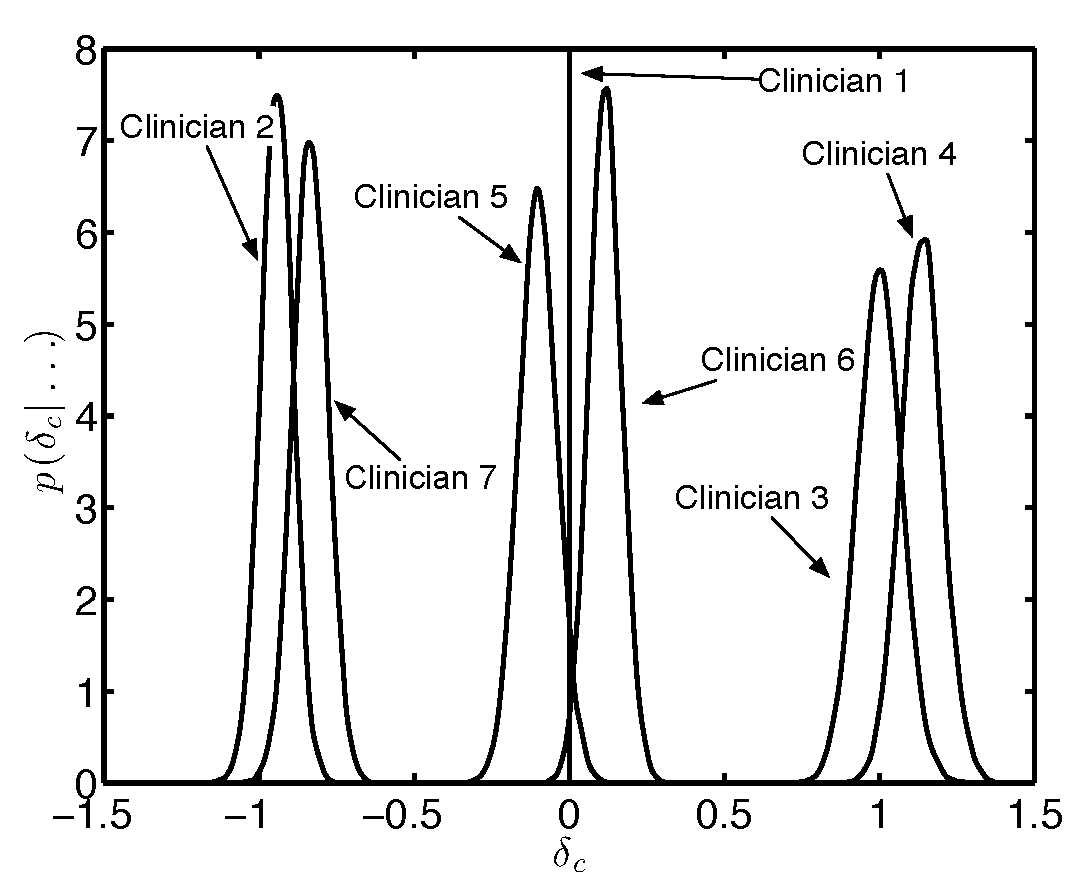
\includegraphics[width=0.8\linewidth]{offset.pdf}
		\centering\caption{\label{fig:offset}Marginal offset posteriors}
	\end{figure}
\end{frame}

\begin{frame}
	\frametitle{Results}
	\begin{figure}[tbh]
		\subfigure[Clinicians 2 and 4]{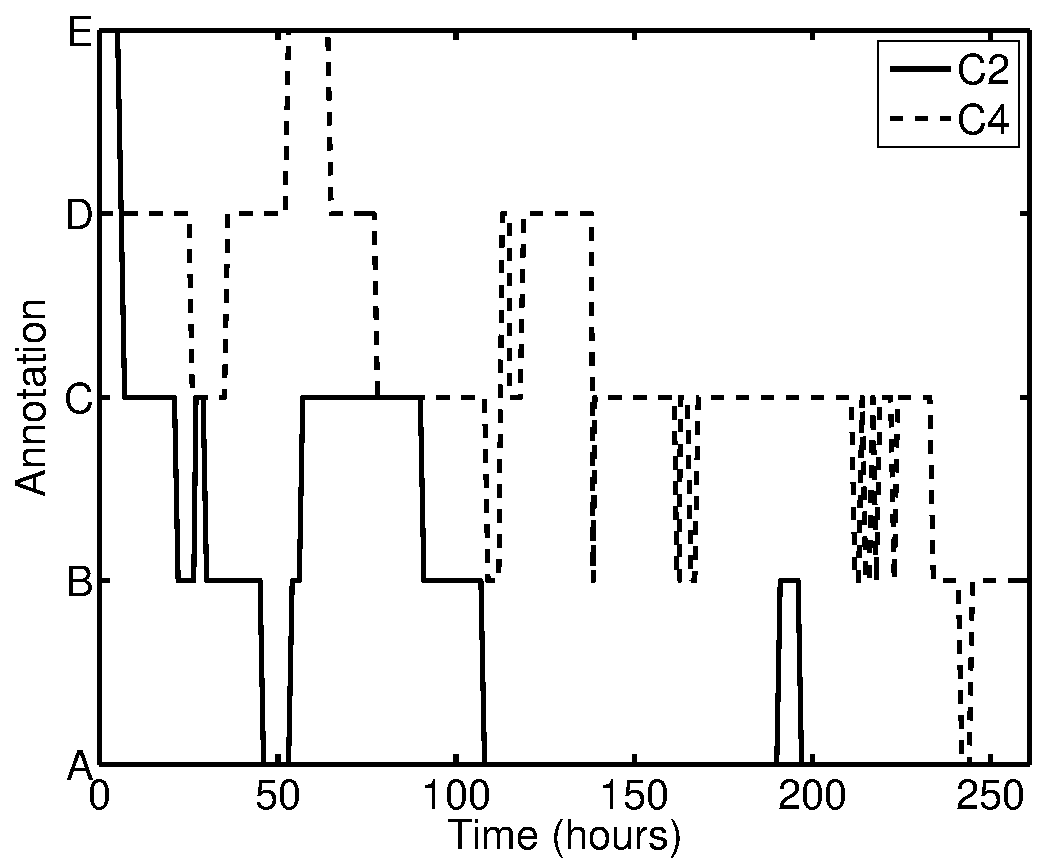
\includegraphics[width=0.45\linewidth]{P2_C24.pdf}}
		\subfigure[Clinicians 3 and 4]{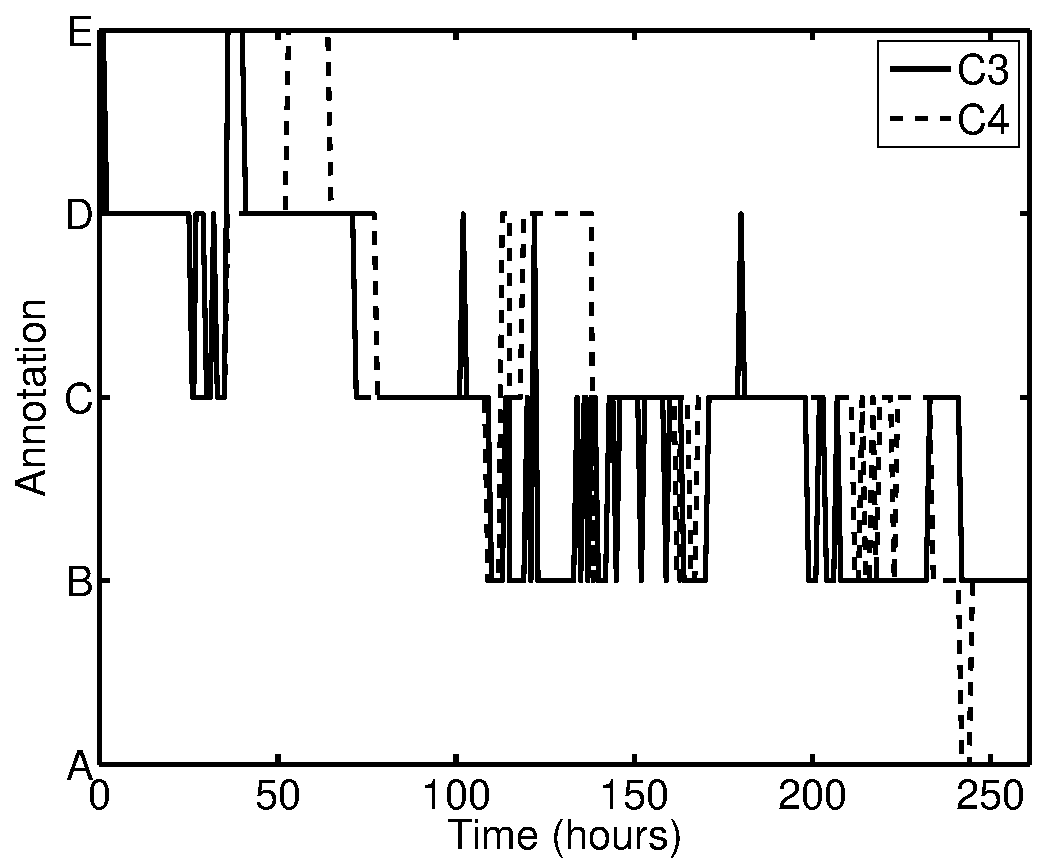
\includegraphics[width=0.45\linewidth]{P2_C34.pdf}}
		\centering\caption{\label{fig:actualratings}Inferred offsets make sense on inspection of the data.}
	\end{figure}
\end{frame}

\begin{frame}
	\frametitle{Results}
	\begin{figure}[tbh]
		\centering\includegraphics[width=0.8\linewidth]{precision_offset_box_17thApril.pdf}
		\centering\caption{\label{fig:clinicalprecision}Marginal precision posteriors. Clinicians 1, 4, and 8 appear to be the least consistent (wrt the majority)}
	\end{figure}
\end{frame}

\begin{frame}
	\frametitle{INSIGHT}
	\begin{itemize}
		\item After the initial annotation, clinicians went through INSIGHT procedure.
		\item The goal was to make ratings more consistent.
		\item If it succeeded, we should see a recuction in offset and increase in precision in the post-INSIGHT data.
	\end{itemize}
\end{frame}

\begin{frame}
	\frametitle{Post-INSIGHT results}
	\begin{figure}[tbh]
		\subfigure[Offsets]{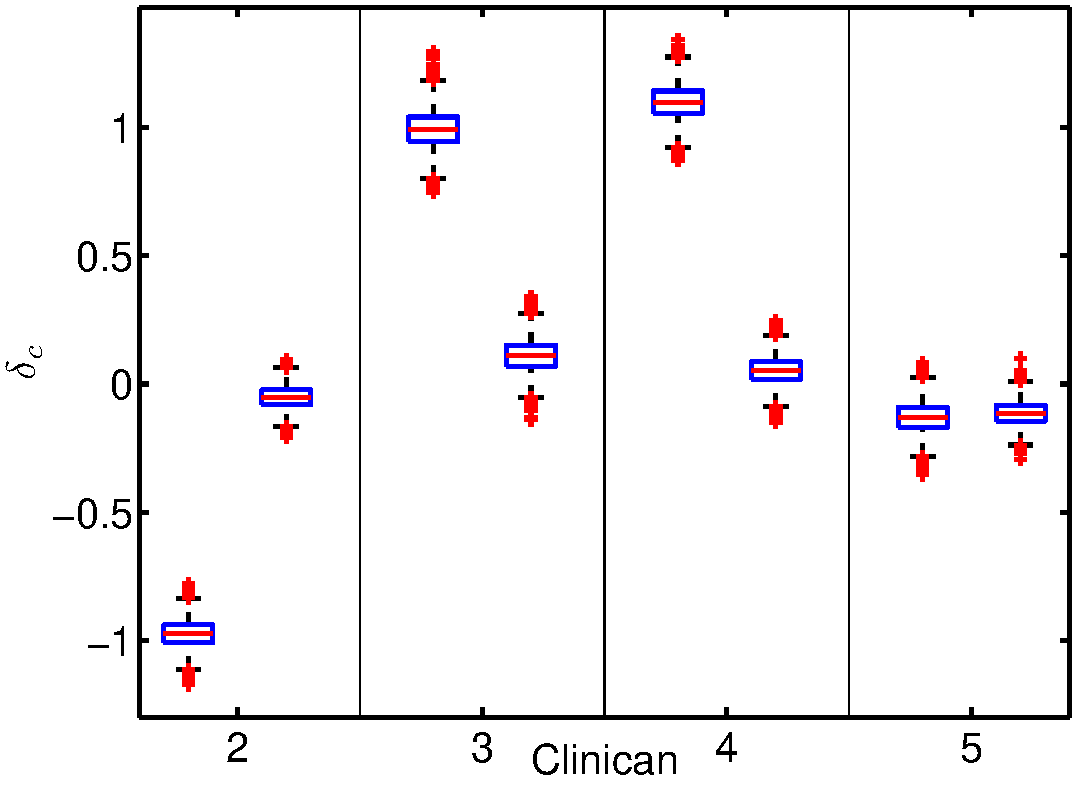
\includegraphics[width=.45\linewidth]{Offset_compare_before_after_17April.pdf}}\hfill
		\subfigure[Precisions]{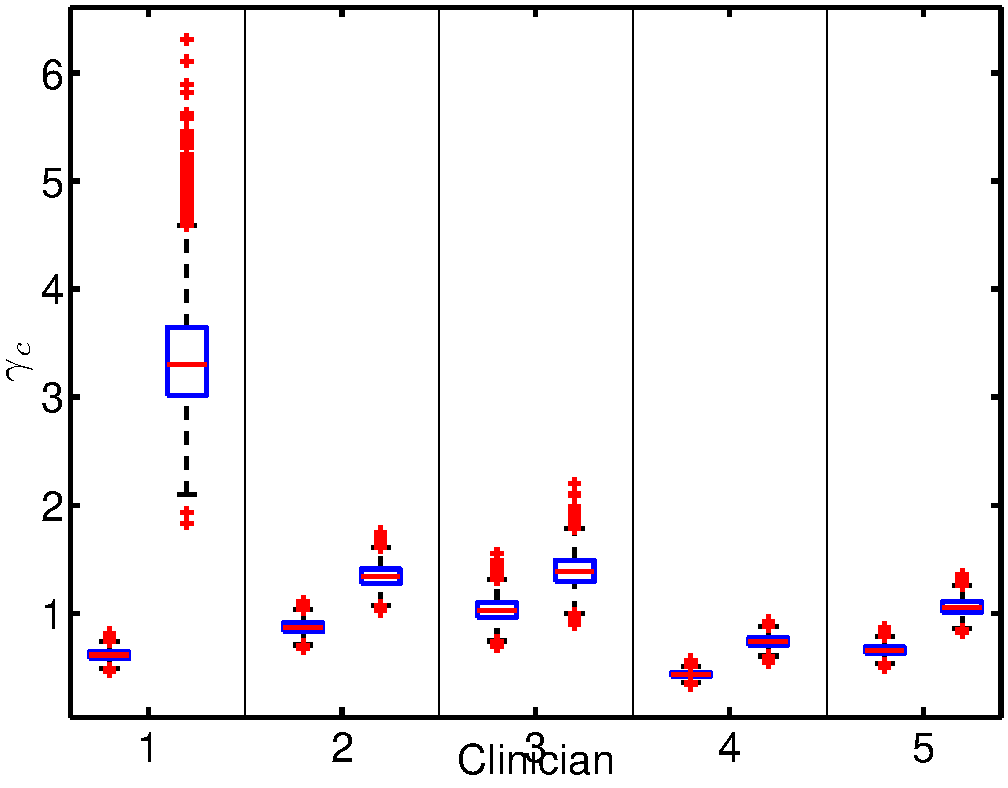
\includegraphics[width=.45\linewidth]{Precision_before_after_April19th.pdf}}
		\centering\caption{\label{fig:clinoffprec}Offsets and precision before and after INSIGHT. Offsets get closer to 0, whilst precision increase suggesting greater agreement amongsth clinicians.}
	\end{figure}
\end{frame}

\begin{frame}
	\frametitle{Inferring category boundaries}
	\begin{itemize}
		\item So far, it has been assumed that all categories are the same size (i.e. the elements of $\mathbf{b}$ are equally spaced).
		\item We can also infer these (with fixed end-points and $\delta_c=0$).
		\item Removes uniform prior assumption over categories.
	\begin{figure}[tbh]
		\subfigure[Before INSIGHT]{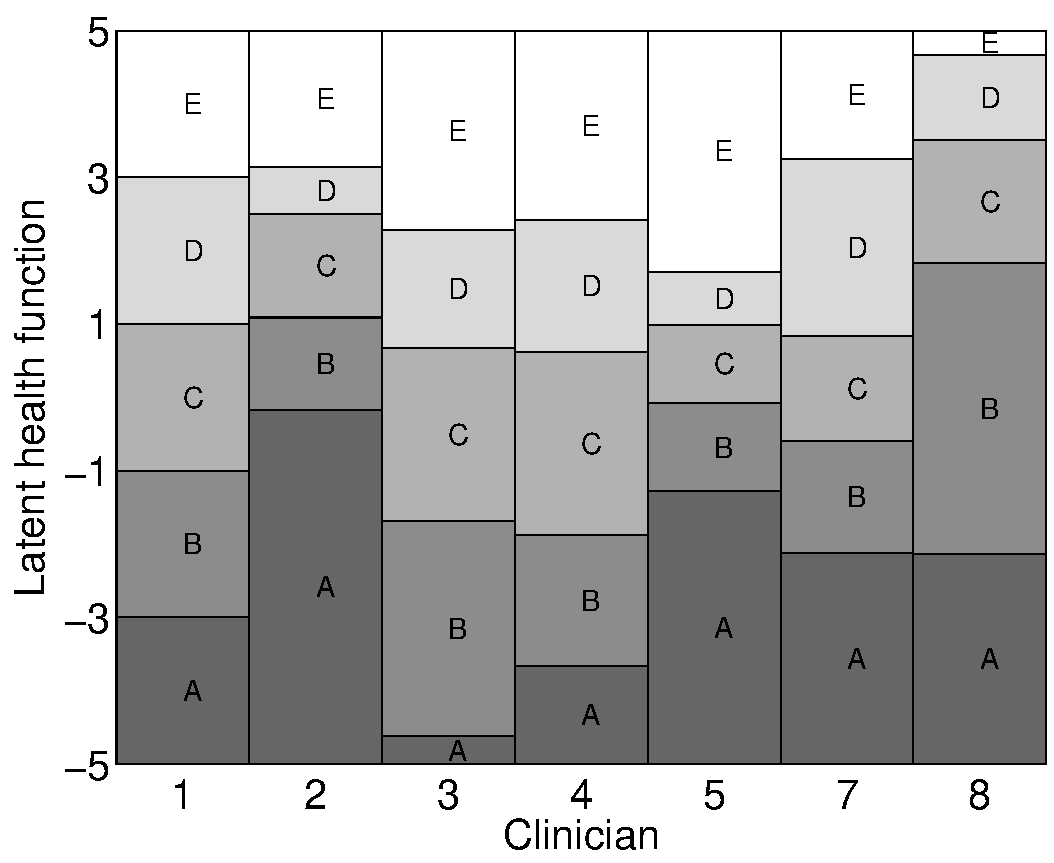
\includegraphics[width=0.45\linewidth]{start_thresh.pdf}}\hfill
		\subfigure[After INSIGHT]{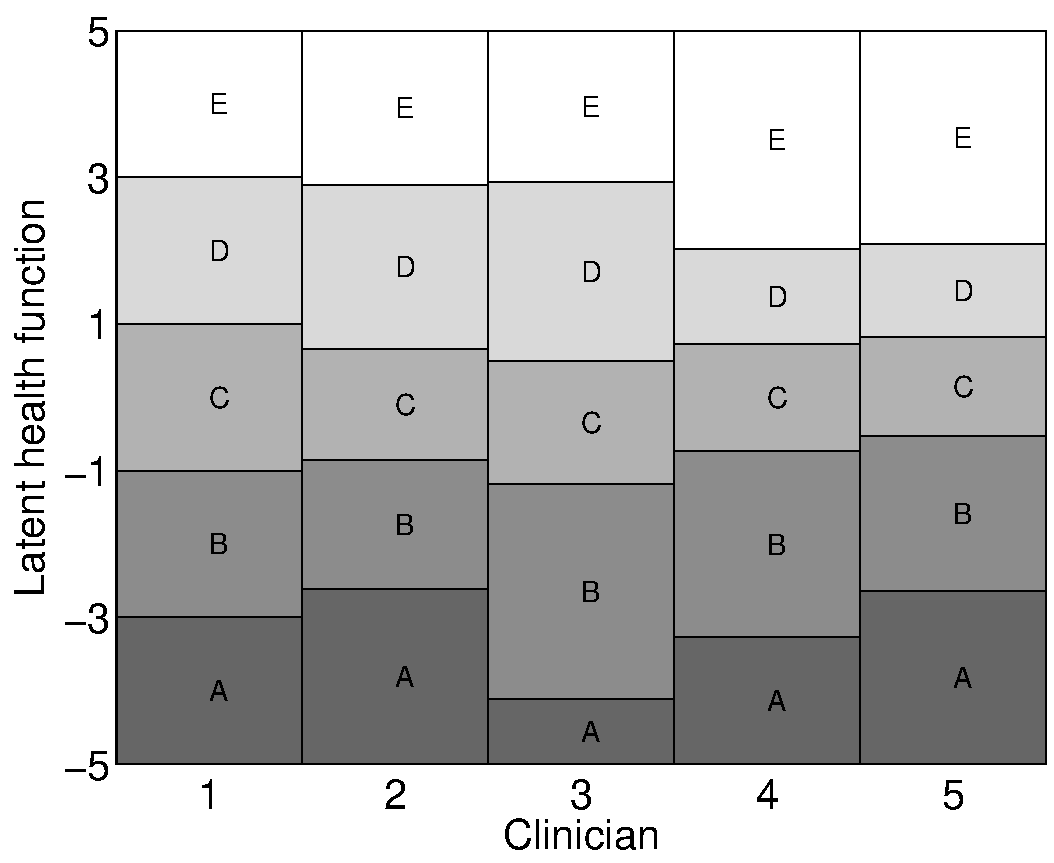
\includegraphics[width=0.45\linewidth]{end_thresh.pdf}}
		\centering\caption{\label{fig:clinicalcategories}Posterior mean cateogory boundaries.}
	\end{figure}
	\end{itemize}
\end{frame}

\begin{frame}
	\frametitle{Summary and Conclusions}
	\begin{itemize}
		\item Model allows us to:
		\begin{itemize}
			\item learn something about \emph{how} clinicians disagree and how they rate.
			\item assess the effectiveness of the INSIGHT procedure.
		\end{itemize}
		\item<2-> GP prior:
		\begin{itemize}
			\item Flexible
			\item Required no parametric assumptions about health function
			\item Hyper-parameter ($\gamma$) was inferred in the model (could be patient-specific)
		\end{itemize}
		\item<3-> Auxiliary Variable Trick:
		\begin{itemize}
			\item Not restricted to a standard Gaussian centered on the GP variable.
			\item Incorporated offset and precision without causing additional inference challenges.
		\end{itemize}
	\end{itemize}
\end{frame}